% ===============================================================
%
%  Template for creating scribe notes for CS:3330, Algorithms.             I am using this template to get my homework PDF's set up as well
%
%  Fill in your name, lecture date, and body of scribe notes
%  as indicated below.
%
% ===============================================================

\documentclass[11pt]{article}

\usepackage{graphicx}
\usepackage{amssymb, amsthm}
\usepackage{pgfplots}
\usepackage{tikz}
\usetikzlibrary{datavisualization}
\usetikzlibrary{datavisualization.formats.functions}
\usepackage{mathtools}
\usepackage{amsmath}



\setlength{\topmargin}{0pt}
\setlength{\textheight}{9in}
\setlength{\headheight}{0pt}
\setlength{\headsep}{0pt}
\setlength{\oddsidemargin}{0.25in}
\setlength{\textwidth}{6in}

\pagestyle{plain}

\begin{document}

\thispagestyle{empty}

\begin{center}
\bf\large CS:3330, Algorithms
\end{center}

\begin{center}
\bf\large HW05 Order Problems    %Fill in Name of Homework here
\end{center}

\noindent
Logan Zweifel     % FILL IN YOUR NAME HERE
\hfill
September 19, 2021           % FILL IN HW DATE HERE

\noindent
\rule{\textwidth}{1pt}

\medskip

%%%%%%%%%%%%%%%%%%%%%%%%%%%%%%%%%%%%%%%%%%%%%%%%%%%%%%%%%%%%%%%%
% BODY OF HOMEWORK NOTES GOES HERE
%%%%%%%%%%%%%%%%%%%%%%%%%%%%%%%%%%%%%%%%%%%%%%%%%%%%%%%%%%%%%%%%

%%%%%%%%%%1 HW4 3
\section{Theta}
Show that $6n^2+12n \in \Theta(n^2)$.

\bigskip
\bigskip
The following is the definition for Theta. For a given complexity function $f(n)$,

\begin{equation*}
\Theta(f(n))= O(f(n))\cap \Omega(f(n))
\end{equation*}

This means that $\Theta(f(n))$ is the set of complexity functions $g(n)$ for which there exists some positive real constants $c_1$ and $c_2$ and some nonnegative integer $N$ such that for all $n \geq N$,

\begin{equation*}
c_1*f(n) \leq g(n) \leq c_2*f(n)
\end{equation*}


\bigskip
\bigskip

\noindent
I show that $6n^2+12n \in \Theta(n^2)$ by using the equations from my work on questions 3 and 6 from HW04, a picture my work for those problems from the previous homework is attached at the end of this question, as they ask to find the Big-O and $\Omega$ of this same function, and because, for $n \geq 1$,
\begin{equation*}
1*n^2 \leq 6n^2+12n \leq 18n^2
\end{equation*}
Where $c_1=1$, $c_2=18$ and $N=1$ were used to obtain the result.

\begin{figure*}[h]
\begin{center}$
\begin{array}{cc}
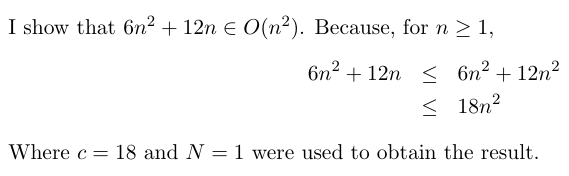
\includegraphics[width=2.5in]{BigO.png} &
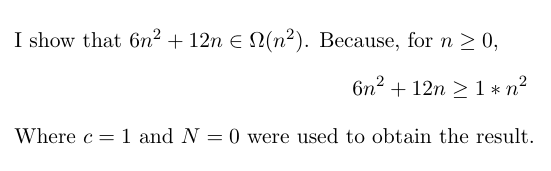
\includegraphics[width=2.5in]{Omega.png}
\end{array}$
\end{center}
\caption{Previous Homework work}
\end{figure*}

%%%%%%%%%%1 HW4
\section{Little-o}
Show directly, using the definition of "Little-o", that $4n \in o(n^2)$.


\bigskip
\bigskip
The following is the definition for "Little-o". For a given complexity function $f(n)$, $o(f(n))$ is the set of complexity functions $g(n)$ satisfying the following: For every positive real constant $c$, there exists a nonnegative integer $N$ such that for all $n \geq N$,

\begin{equation*}
g(n) \leq c * f(n)
\end{equation*}


\bigskip
\bigskip
\noindent

I show that $4n \in o(n^2)$ by first assuming that $c>0$ which is given by the definition of "Little-o". Now, I need to find the valid N values.
\begin{eqnarray*}
4n &\leq& c*n^2 \\
\frac{4}{c} &\leq& n
\end{eqnarray*}
Therefore, you can choose any $N \geq \frac{4}{c}$. For this problem, the valid values for N are dependent on the value of the constant $c$.



%%%%%%%%%%1 HW4 5
\section{Little-w}
Show directly, using the definition of "Little-$\omega$", that $4n^3 \in \omega(n)$.

\bigskip
\bigskip
The following is the definition for "Little-$\omega$". For a given complexity function $f(n)$, $\omega(f(n))$ is the set of complexity functions $g(n)$ satisfying the following: For every positive real constant $c$, there exists a nonnegative integer $N$ such that for all $n \geq N$,

\begin{equation*}
g(n) \geq c * f(n)
\end{equation*}


\bigskip
\bigskip
I show that $4n^3 \in \omega(n)$ by first assuming that $c>0$ which is given by the definition of "Little-$\omega$". Now, I need to find a valid N value.
\begin{eqnarray*}
4n^3 &\geq& c*n \\
4n^2 &\geq& c\\
2n &\geq& \sqrt{c}\\
n &\geq& \frac{\sqrt{c}}{2}
\end{eqnarray*}
Therefore, you can choose any $N \geq \frac{\sqrt{c}}{2}$. For this problem, the valid values for N are dependent on the value of the constant $c$.


%%%%%%%%%%1
\section{Big-O}
Show directly, using the definition of Big-O, that for all $a,b, >1$,  $log_a(n) \in O(log_b(n))$.

\bigskip
\bigskip

The following is the definition for Big-O. For a given complexity function $f(n)$, $O(f(n))$ is the set of complexity functions $g(n)$ for which there exists some positive real constant $c$ and some nonnegative integer $N$ such that for all $n \geq N$,

\begin{equation*}
g(n) \leq c * f(n)
\end{equation*}

\bigskip
\bigskip

In addition, Both this question and the next one will use the logarithm change of base formula which is the following:
\begin{equation*}
log_b(x) = \frac{log_c(x)}{log_c(b)}
\end{equation*}

\bigskip
\bigskip

The following was done using the definition of Big-O and the logarithm change of base formula and for $n \geq 1$:

\begin{eqnarray*}
log_a(n) &\leq& c*log_b(n) \\
log_a(n) &\leq& c*\frac{log_a(n)}{log_a(b)} \\
\frac{log_a(n)}{log_a(n)} &\leq& c*\frac{1}{log_a(b)} \\
1 &\leq& \frac{c}{log_a(b)} \\
log_a(b) &\leq& c
\end{eqnarray*}
Essentially, this shows that for N=1, the valid constant values that can satisfy the definition of Big-O is directly related to the integers a and b.


%%%%%%%%%%%2
\section{Omega}
Show directly, using the definition of $\Omega$, that for all $a,b, >1$,  $log_a(n) \in \Omega(log_b(n))$.

\bigskip
\bigskip
The following is the definition for Omega. For a given complexity function $f(n)$, $\Omega(f(n))$ is the set of complexity functions $g(n)$ for which there exists some positive real constant $c$ and some nonnegative integer $N$ such that for all $n \geq N$,

\begin{equation*}
g(n) \geq c * f(n)
\end{equation*}

\bigskip
\bigskip
The following was done using the definition of Omega and the logarithm change of base formula defined in the previous problem. For $n \geq 1$:

\begin{eqnarray*}
log_a(n) &\geq& c*log_b(n) \\
log_a(n) &\geq& c*\frac{log_a(n)}{log_a(b)} \\
\frac{log_a(n)}{log_a(n)} &\geq& c*\frac{1}{log_a(b)} \\
1 &\geq& \frac{c}{log_a(b)} \\
log_a(b) &\geq& c
\end{eqnarray*}
Just as the previous problem did, the valid values for the constant c to satisfy the definition of Omega are dependent on the values of a and b.


%%%%%%%%%3
\section{Theta}
Show that for all $a,b, >1$,  $log_a(n) \in \Theta(log_b(n))$.

\bigskip
\bigskip
The following is the definition for Theta. For a given complexity function $f(n)$,

\begin{equation*}
\Theta(f(n))= O(f(n))\cap \Omega(f(n))
\end{equation*}

This means that $\Theta(f(n))$ is the set of complexity functions $g(n)$ for which there exists some positive real constants $c_1$ and $c_2$ and some nonnegative integer $N$ such that for all $n \geq N$,

\begin{equation*}
c_1*f(n) \leq g(n) \leq c_2*f(n)
\end{equation*}

\bigskip
I show that for all $a,b, >1$,  $log_a(n) \in \Theta(log_b(n))$ by using the work done in problems 1 and 2 to satisfy the conditions of Theta. For $N=1$ and $c_1 \leq log_a(b) \leq c_2$,

\begin{equation*}
c_1*log_b(n) \leq log_a(n) \leq c_2*log_b(n)
\end{equation*}

The constants in this solution can not be explicitly defined as they are dependent on the values of a and b. However, given the relationship stated earlier between both constant and $log_a(b)$ there is a defined range of valid constant values for any given N, therefore showing that $log_a(n) \in \Theta(log_b(n))$.

%%%%%%%%%%%%4
\section{Theta using limits}
Use limits to show $13n^2+7n+\sqrt2 \in \Theta(n^2)$


\bigskip
\bigskip

This problem uses Theorem 1.3 from the book which is property 13 on the propertiesoforder.pdf. That property/theorem is the following:

\[ \lim\limits_{n \to \infty} \frac{g(n)}{f(n)} =
  \begin{cases}
    c       & \quad \text{implies }  g(n) \text{$\in \Theta (f(n))$, if $c>0$}\\
    0       & \quad \text{implies } g(n) \text{$\in o(f(n))$}\\
    \infty  & \quad \text{implies } f(n) \text{$\in o(g(n))$}
  \end{cases}
\]

Applying this limit rule to this specific problem results in the following:
\begin{eqnarray*}
\lim\limits_{n \to \infty} \frac{g(n)}{f(n)} &=& \lim\limits_{n \to \infty} \frac{13n^2+7n+\sqrt2}{n^2} \\
&=& \lim\limits_{n \to \infty} \frac{13n^2}{n^2} \\
&=& 13 * \lim\limits_{n \to \infty} \frac{n^2}{n^2} \\
&=& 13
\end{eqnarray*}
In the second line of these equations, I am allowed to drop the lower degree terms, and only have $13n^2$ on top because as a function moves towards infinity, a higher degree term will dominate the lower terms and then I can pull 13 from within the limit as it is a constant. The result of this limit is a constant greater than 0, 13, and therefore I have shown that $13n^2+7n+\sqrt2 \in \Theta (n^2)$.


%%%%%%%%%%%5
\section{$t(n)$}
Consider the function

\[ t(n) =
  \begin{cases}
    2n       & \quad \text{if } n \text{ is even}\\
    1  & \quad \text{if } n \text{ is odd}
  \end{cases}
\]

\subsection*{a) Show that $t(n) \in O(n) - \Omega(n)$}
A function that is $t(n) \in O(n) - \Omega(n)$ is a function that is $O(f(n)$, but is not $\Omega (f(n))$. First, I will show that $t(n)$ is $O(n)$. Referring to the definition of Big-O stated in problem 1, for $n \geq 0$ and all subsequent even n values exclusively (first case of $t(n)$),

\begin{equation*}
2n \leq 3*n \equiv 2n \leq 3n
\end{equation*}
Where $c=3$ and $N=0$ were used to obtain the first case of $t(n)$. For the second case where values of n are odd, the same values for $c$ and $N$ will be used to prove both cases work for these numbers.

\begin{equation*}
1 \leq 3n
\end{equation*}
As I have proved both cases of $t(n)$ are in $O(n)$, $t(n)$ as a complete function must be $O(n)$ as well.

\bigskip
Referring to the definion of Omega stated in problem 2, $t(n)$ can't be $\Omega (n)$ as for any value of $c$ no matter how small, $c*n$ will eventually be greater than 1 and not satisfy the definition of Omega when n is an odd number.

\bigskip
I have shown that $t(n)$ is $O(n)$ and is not $\Omega (n)$ and have therefore proved that $t(n) \in O(n) - \Omega(n)$.


\subsection*{b) Show that $t(n) \notin o(n)$}
I will show that $t(n) \notin o(n)$ by using a proof by contradiction. Let c=1. If $t(n) \in o(n)$, then there must exist some $N$ such that, for $n \geq N$,

\begin{equation*}
t(n) \leq 1*n \equiv t(n) \leq n
\end{equation*}

This equality is not true for all even n values greater than 0. This contradiction proves that $t(n) \notin o(n)$.














%%%%%%%%%%%%%%%%%%%%%%%%%%%%%%%%%%%%%%%%%%%%%%%%%%%%%%%%%%%%%%%%

\end{document}

